\documentclass[aspectratio=169]{beamer}
\usepackage[utf8]{inputenc}
\usepackage{lmodern}
\usepackage{amsmath,amssymb}
\usepackage{booktabs}
\usepackage{array}
\usepackage{xcolor}
\usepackage{mathpartir}
\usepackage{tikz}
\usetikzlibrary{arrows.meta,positioning,fit,calc,backgrounds,shapes.geometric}
\usepackage{pgfplots}
\pgfplotsset{compat=1.18}

\usetheme{CambridgeUS}
\usefonttheme{serif}
\setbeamertemplate{navigation symbols}{}
\setbeamertemplate{headline}{}
\setbeamertemplate{footline}[frame number]
\setbeamerfont{block title}{size=\small}

\newcolumntype{L}[1]{>{\raggedright\arraybackslash}p{#1}}
\definecolor{newc}{RGB}{0,120,60}
\definecolor{oldc}{RGB}{110,110,110}
\definecolor{lcc}{RGB}{150,60,20}
\newcommand{\opt}[1]{\texttt{#1}}
\newcommand{\sm}[1]{\texttt{#1}}
\newcommand{\TC}{\mathit{TC}}
\newcommand{\cyc}[1]{\mathsf{cyclic}(#1)}
\newcommand{\fun}[1]{\mathsf{fun}(#1)}
\newcommand{\rn}[1]{\textsc{#1}}
\newcommand{\new}[1]{\textcolor{newc}{#1}}
\newcommand{\good}[1]{\textcolor{green!45!black}{#1}}
\newcommand{\bad}[1]{\textcolor{red!70!black}{#1}}
\newcommand{\tmo}{\textcolor{gray}{timeout}}
\newcommand{\best}[1]{\textbf{\good{#1}}}
\newcommand{\pfTimeout}{300}
\newcommand{\pfVirtual}{13}
\newcommand{\pfReal}{13}
\newcommand{\pfTotal}{13}
\newcommand{\pfWrong}{0}
\newcommand{\pfSame}{12}
\newcommand{\pfRatioMin}{0.69}
\newcommand{\pfRatioMax}{1.24}
\newcommand{\pfRatioMed}{0.96}
\newcommand{\pfMaxReal}{79.5}
\newcommand{\pfNumConfigs}{7}
\newcommand{\pfJobs}{6}
\newcommand{\pfBestSingle}{12}
\newcommand{\pfBestSingleName}{FMF+R}
\newcommand{\pfCvc}{6094bb5747}
\newcommand{\pfBench}{e4a4f7e}


\tikzset{
  box/.style={rectangle,draw,rounded corners,thick,align=center,inner sep=3pt,font=\footnotesize},
  stp/.style={rectangle,draw,rounded corners=2pt,minimum width=3.0cm,minimum height=5mm,
               inner sep=1pt,font=\scriptsize\ttfamily},
  newstp/.style={stp,fill=newc!15,draw=newc,thick},
  rules/.style={rectangle,draw=gray!60,rounded corners=2pt,align=left,inner sep=3pt,font=\scriptsize},
  ev/.style={circle,draw,thick,minimum size=7mm,inner sep=0pt,font=\small},
  arr/.style={->,thick,>=Stealth},
  lab/.style={font=\scriptsize,inner sep=1pt},
}
\mprset{sep=1.6em}

\title[Cycles and functionality in cvc5's relations solver]{Cycles and Functionality in cvc5's Relations Solver}
\subtitle{\texttt{rel.cyclic}, \texttt{rel.is-functional} and their calculus\\[1mm]
  \small the pull request to cvc5 main (branch \texttt{cycle-ext-cyclic})}
\author{}
\institute{}
\date{October 2026}

\begin{document}

\frame{\titlepage}

\begin{frame}{Outline}
  \tableofcontents
\end{frame}

%=====================================================================
\section{Motivation}

\begin{frame}[fragile]{Relational specifications need acyclicity and functionality}
  \begin{columns}[T]
  \begin{column}{0.52\textwidth}
    \small
    \textbf{Axiomatic memory models} allow an execution iff some union of relations is acyclic,
    e.g.\ sequential consistency: $\mathit{po}\cup\mathit{rf}\cup\mathit{co}\cup\mathit{fr}$ is acyclic.
    \textbf{Alloy-style specifications} constrain relations to be (partial) functions.
    \medskip

    \textbf{In cvc5 main} both properties must be stated with quantifiers:
    \[
      \begin{array}{l}
        \forall x.\ (x,x)\notin \TC(R) \\[1mm]
        \forall x\,y\,z.\ (x,y)\in R \wedge (x,z)\in R \Rightarrow y = z
      \end{array}
    \]
    and the negation of acyclicity needs an existential witness. Instantiation (E-matching or
    finite model finding) has to find the right instances.
  \end{column}
  \begin{column}{0.46\textwidth}
    \small
    \textbf{With this PR}, two predicates that the relations solver reasons about directly:
    \begin{block}{}
    \footnotesize
\begin{verbatim}
; a forbidden execution: a cycle
(assert (rel.cyclic
  (set.union po (set.union rf
    (set.union co fr)))))
; po is acyclic and functional
(assert (not (rel.cyclic po)))
(assert (rel.is-functional po))
\end{verbatim}
    \end{block}
    No quantifier for acyclicity or functionality; a calculus of inference rules
    instead (this talk).
  \end{column}
  \end{columns}
\end{frame}

\begin{frame}{The benchmarks: completeness of litmus-test templates}
  \begin{columns}[T]
  \begin{column}{0.55\textwidth}
    \small
    13 memory-model benchmarks (relational-solver-benchmarks): SC, SC per location (plsc),
    TSO; one and two threads; variants \sm{just-rf} and \sm{no-ltts}.
    \medskip

    Each asks: \emph{is there an execution that violates the memory model but that no
    litmus-test template forbids?}
    \begin{itemize}
      \item \sm{unsat}: the templates are complete (10 files);
      \item \sm{sat}: cvc5 prints such an execution (3 files).
    \end{itemize}
    The violation is a cycle: \sm{(rel.cyclic (set.union po rf co fr))}; the templates and the
    model are acyclicity and functionality constraints on the derived relations.
  \end{column}
  \begin{column}{0.43\textwidth}
    \centering
    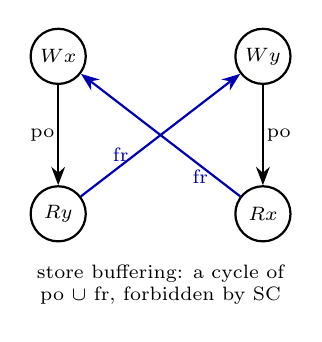
\begin{tikzpicture}[x=1cm,y=1cm]
      \node[ev] (w1) at (0,2) {\scriptsize $W x$};
      \node[ev] (r1) at (0,0) {\scriptsize $R y$};
      \node[ev] (w2) at (2.6,2) {\scriptsize $W y$};
      \node[ev] (r2) at (2.6,0) {\scriptsize $R x$};
      \draw[arr] (w1) -- node[lab,left]{po} (r1);
      \draw[arr] (w2) -- node[lab,right]{po} (r2);
      \draw[arr,blue!70!black] (r1) -- node[lab,pos=0.25,above]{fr} (w2);
      \draw[arr,blue!70!black] (r2) -- node[lab,pos=0.25,below]{fr} (w1);
      \node[font=\scriptsize,align=center] at (1.3,-0.9) {store buffering: a cycle of\\
        po $\cup$ fr, forbidden by SC};
    \end{tikzpicture}
  \end{column}
  \end{columns}
\end{frame}

%=====================================================================
\section{What is new compared to cvc5 main}

\begin{frame}{The changes at a glance}
  \scriptsize
  \begin{tabular}{@{}lL{11.2cm}@{}}
    \toprule
    component & change \\
    \midrule
    kinds, API & \new{\sm{RELATION\_CYCLIC}} (\sm{rel.cyclic}), \new{\sm{RELATION\_IS\_FUNCTIONAL}}
      (\sm{rel.is-functional}), \sm{RELATION\_RCLOSURE}, \sm{RELATION\_RTCLOSURE}
      (\sm{rel.rclosure}, \sm{rel.rtclosure}); parser, printer, CPC signature \\
    type rules & a binary relation whose columns have the same sort (cyclic, closures);
      any binary relation (functional) \\
    rewriter & evaluation and elimination rules (constants, empty set, singletons, unions) \\
    relations solver & \new{the calculus}: cycle witness, minimality, acyclicity, anchors,
      closure induction, functionality, lazy closure splits, grounding conflicts \\
    strategy & a new full-effort step, three last-call steps, \sm{needsCheckLastEffort} \\
    options & \sm{--rels-functional-mode}, \sm{--rels-acyclic-anchor},
      \sm{--rels-acyclic-backward-chords}, \sm{--rels-tc-subset}, \sm{--rels-tc-down-lazy},
      \sm{--rels-acyclic-hammer} \\
    defaults & MiniSat under \sm{--sets-exp} (justification heuristic), except for sygus-style problems \\
    fixes & closure rules (edge explanations, conclusions on the tuple of the explanation);
      no redundant facts in the sets solver \\
    tests, docs & 53 regression files; \sm{docs/theories/sets-and-relations.rst} \\
    \bottomrule
  \end{tabular}
  \medskip

  Against cvc5 main (a3f47bdffd): 28 source files, $+3305/-131$ lines; tests $+1958$ lines.\\
  \sm{scripts/} (experiment scripts, these slides) is temporary.
\end{frame}

\begin{frame}{New predicates}
  \begin{columns}[T]
  \begin{column}{0.5\textwidth}
    \begin{block}{\sm{(rel.cyclic R)}, \ $R$ : \sm{(Relation T T)}}
      \small
      \[ \cyc{R} \iff \exists x.\ (x,x)\in R^{+} \]
      Acyclicity is \sm{(not (rel.cyclic R))}.\\[1mm]
      e.g.\ \sm{(rel.cyclic (set.union R S))} holds for $R=\{(a,b)\}$, $S=\{(b,a)\}$;
      \sm{(rel.cyclic R)} and \sm{(rel.cyclic S)} do not.
    \end{block}
    \begin{block}{\sm{(rel.is-functional R)}, \ $R$ : \sm{(Relation T1 T2)}}
      \small
      \[ \fun{R} \iff \forall x\,y\,z.\ (x,y),(x,z)\in R \Rightarrow y=z \]
      Right-unique, not necessarily total.
    \end{block}
  \end{column}
  \begin{column}{0.48\textwidth}
    \begin{block}{\sm{(rel.rclosure R)}, \sm{(rel.rtclosure R)}}
      \small
      $R$ plus $(x,x)$ for every $x$ in its domain or range; and that union with
      $R^{+}$. Eliminated by rewriting when $R$ is built from $\emptyset$, singletons and
      unions; otherwise the solver answers \sm{unknown}.
    \end{block}
    \small
    \textbf{Why a predicate and not a definition?} The definitions need a quantifier (or the
    universe set, which cvc5 does not interpret as all elements). As predicates, the solver
    builds \emph{witnesses} and \emph{explanations} for them, and uses their structure
    (unions, closures, joins) in its rules.
  \end{column}
  \end{columns}
\end{frame}

\begin{frame}{Rewrite rules: what holds in every context}
  \small
  The rewriter only replaces a term by an \emph{equivalent} term, independently of the
  assertions:
  \begin{center}\scriptsize\setlength{\tabcolsep}{4pt}
  \begin{tabular}{@{}lll@{}}
    \toprule
    term & rewritten to & why \\
    \midrule
    \sm{(rel.cyclic $\emptyset$)} & \sm{false} & no pair at all \\
    \sm{(rel.cyclic \{(x,y)\})} & \sm{(= x y)} & only a self-loop \\
    \sm{(rel.cyclic $c$)}, $c$ constant & \sm{true} / \sm{false} & evaluate $c^{+}$ \\
    \midrule
    \sm{(rel.is-functional X)}, $X$: $\emptyset$, \sm{\{t\}}, \sm{(rel.iden A)} & \sm{true} & at most one image \\
    \sm{(rel.is-functional $c$)}, $c$ constant & \sm{true} / \sm{false} & first components \\
    \midrule
    \sm{(rel.rclosure \{(x,y)\})} & $\{(y,y)\}\cup(\{(x,x)\}\cup\{(x,y)\})$ & definition \\
    \sm{(rel.rclosure (set.union A B))} & \sm{(rel.rclosure A)} $\cup$ \sm{(rel.rclosure B)} & union \\
    \sm{(rel.rtclosure R)} & \sm{(rel.rclosure R)} $\cup$ \sm{(rel.tclosure R)} & definition \\
    \bottomrule
  \end{tabular}
  \end{center}
  Everything else is done by \emph{inference rules} in the relations solver (next section).
\end{frame}

%=====================================================================
\section{The calculus}

\begin{frame}{Notation}
  \begin{columns}[T]
  \begin{column}{0.55\textwidth}
    \small
    \begin{itemize}
      \item A configuration: the asserted literals and the equivalence classes of the
        equality engine; $t \sim t'$: equal in the current context.
      \item A rule
        \(\inferrule{P_1 \\ \dots \\ P_n}{C}\)
        sends the \emph{lemma} $P_1\wedge\dots\wedge P_n \Rightarrow C$, a valid clause whose
        premises are the explanation (used by conflict analysis, unsat cores and proofs).
      \item Fresh symbols are skolems, cached by their key, so each is created once.
      \item The \emph{cycle witness} of $\cyc{R_1\cup\dots\cup R_k}$: elements
        $s_1,\dots,s_l$ with $s_l = s_1$ ($l-1$ edges), each edge in some $\TC(R_j)$.
    \end{itemize}
  \end{column}
  \begin{column}{0.43\textwidth}
    \centering
    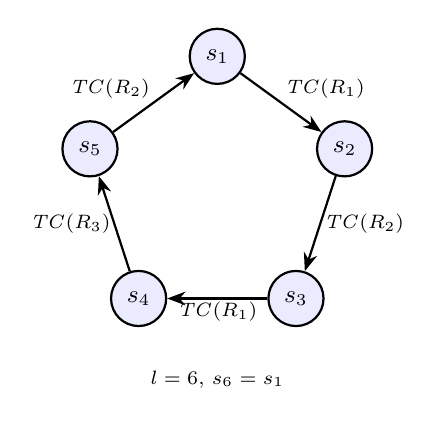
\begin{tikzpicture}
      \foreach \i/\a in {1/90,2/18,3/-54,4/-126,5/162} {
        \node[ev,fill=blue!8] (s\i) at (\a:1.7cm) {$s_{\i}$};
      }
      \draw[arr] (s1) -- node[lab,above right]{$\TC(R_1)$} (s2);
      \draw[arr] (s2) -- node[lab,right]{$\TC(R_2)$} (s3);
      \draw[arr] (s3) -- node[lab,below]{$\TC(R_1)$} (s4);
      \draw[arr] (s4) -- node[lab,left]{$\TC(R_3)$} (s5);
      \draw[arr] (s5) -- node[lab,above left]{$\TC(R_2)$} (s1);
      \node[font=\scriptsize] at (0,-2.4) {$l = 6$, $s_6 = s_1$};
    \end{tikzpicture}
  \end{column}
  \end{columns}
\end{frame}

\begin{frame}{Cyclicity: creating and unrolling the witness}
  \small\mprset{sep=1.2em}\vspace{-2mm}
  For an asserted $\cyc{R}$ (fresh $s$, $s_1$, $l$, $s_{i+1}$):
  \begin{mathpar}
    \inferrule*[right=\rn{Cycle-Def}]{\cyc{R} \\ R \text{ not a union}}{(s,s)\in \TC(R)}
    \and
    \inferrule*[right=\rn{Inst-Cycle}]{\cyc{R_1\cup\dots\cup R_k}}{1 < l}
    \\
    \inferrule*[right=\rn{Unroll}]{\cyc{R} \\ i < l}
      {(s_i,s_{i+1})\in \TC(R_1)\ \vee\ \dots\ \vee\ (s_i,s_{i+1})\in \TC(R_k)}
    \and
    \inferrule*[right=\rn{Split-Len}]{\cyc{R} \\ i \le l}{i < l\ \vee\ (l = i \wedge s_i = s_1)}
    \and
    \inferrule*[right=\rn{Same-Operands}]{\cyc{R'} \\ R' \text{ has the operands of } R}
      {\cyc{R}}
  \end{mathpar}
  \footnotesize
  \begin{itemize}
    \item The operands of nested unions are flattened: the witness of
      $\cyc{rf\cup(po\cup co)}$ alternates between $\TC(rf)$, $\TC(po)$, $\TC(co)$.
    \item One \rn{Unroll} per check round; at last call the witness is completed to the value
      of $l$ in the candidate model.
  \end{itemize}
\end{frame}

\begin{frame}{Minimality: the witness is a shortest cycle}
  \begin{columns}[T]
  \begin{column}{0.6\textwidth}
    \footnotesize\mprset{sep=1.2em}
    A shortest cycle of $\TC(R_1)\cup\dots\cup\TC(R_k)$ exists whenever a cycle does, so the
    witness can be assumed shortest (for $q<r\le l$, every $R_j$):
    \begin{mathpar}
      \inferrule*[right=\rn{Alternate}]{\cyc{R} \\ i < l}
        {\neg\big((s_{i-1},s_i)\in\TC(R_j) \wedge (s_i,s_{i+1})\in\TC(R_j)\big)}
      \\
      \inferrule*[right=\rn{Chord}]{\cyc{R} \\ r \le l \\ q < r-1 \\ (q,r)\ne(1,l)}
        {(s_q,s_r)\notin\TC(R_j)}
      \\
      \inferrule*[right=\rn{Distinct}]{\cyc{R} \\ r \le l \\ (q,r)\ne(1,l)}{s_q \ne s_r}
    \end{mathpar}
    \textbf{\rn{Backward}} (\sm{--rels-acyclic-backward-chords}): $(s_r,s_q)\notin\TC(R_j)$ if it
    closes a shorter cycle. It lets a totality axiom (e.g.\ $po$ within a thread) bound the
    length of the witness.
  \end{column}
  \begin{column}{0.38\textwidth}
    \centering
    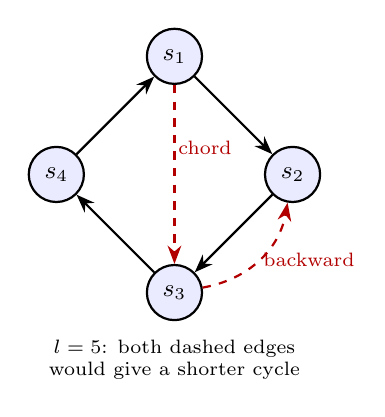
\begin{tikzpicture}
      \foreach \i/\a in {1/90,2/0,3/-90,4/180} {
        \node[ev,fill=blue!8] (s\i) at (\a:1.5cm) {$s_{\i}$};
      }
      \draw[arr] (s1) -- (s2);
      \draw[arr] (s2) -- (s3);
      \draw[arr] (s3) -- (s4);
      \draw[arr] (s4) -- (s1);
      \draw[arr,dashed,red!70!black] (s1) -- node[lab,right,pos=0.35]{chord} (s3);
      \draw[arr,dashed,red!70!black] (s3) to[bend right=35] node[lab,right]{backward} (s2);
      \node[font=\scriptsize,align=center] at (0,-2.35) {$l=5$: both dashed edges\\would give a shorter cycle};
    \end{tikzpicture}
  \end{column}
  \end{columns}
\end{frame}

\begin{frame}{Acyclicity}
  \small\vspace{-2mm}
  For an asserted $\neg\cyc{u}$:
  \begin{mathpar}
    \inferrule*[right=\rn{Acyclic-Down}]{(a,b)\in\TC(R) \\ \neg\cyc{u} \\ u \sim R}{a \ne b}
    \and
    \inferrule*[right=\rn{Register}]{\neg\cyc{u}}{u \subseteq \TC(u)}
  \end{mathpar}
  \begin{itemize}
    \item \rn{Acyclic-Down} turns every reflexive closure membership into a conflict. The
      existing closure rules produce those memberships:
      {\footnotesize
      \begin{mathpar}
        \inferrule*[right=\rn{TC-Up}]{(a,b)\in R \\ (b,c)\in \TC(R)}{(a,c)\in\TC(R)}
        \and
        \inferrule*[right=\rn{TC-Down}]{(a,b)\in\TC(R)}{(a,b)\in R \vee \big((a,k_1),(k_2,b)\in R
          \wedge (k_1 = k_2 \vee (k_1,k_2)\in\TC(R))\big)}
      \end{mathpar}}
    \item \rn{Register} is valid and does nothing logically: it makes $\TC(u)$ a term of the
      solver even if the input never mentions it, so that a cycle of $u$ is found.
    \item The conclusion is stated on the tuple of the explanation, not on its representative
      (the lemma is context-independent).
  \end{itemize}
\end{frame}

\begin{frame}{Cyclic meets acyclic: anchor rules}
  \begin{columns}[T]
  \begin{column}{0.6\textwidth}
    \small
    A cycle of $R$ all of whose edges lie in $\TC(S)$ would be a cycle of $S$:
    \begin{mathpar}
      \inferrule*[right=\rn{Inclusion}]{\cyc{R} \\ \neg\cyc{S}}
        {t\in R' \wedge t \notin \TC(S)}
      \\
      \inferrule*[right=\rn{Branch}]{\cyc{R} \\ \neg\cyc{S} \\ l = N}
        {\textstyle\bigvee_{i<N} (s_i,s_{i+1})\notin\TC(S)}
    \end{mathpar}
    $t$ fresh; $R'$: the operands of $R$ \emph{not} syntactically in $\TC(S)$ (e.g.\
    $S\cap Y$, $\TC(S)$, $S;S$ are). If there is none, the lemma is \sm{false}.
    \medskip

    \rn{Branch} is sent at last call, with $N$ the value of $l$ in the candidate model; with
    $l=N$ in its premises the listed edges are the whole cycle. \sm{--rels-acyclic-anchor}:
    \sm{branch} (default), \sm{inclusion}, \sm{both}, \sm{none}.
  \end{column}
  \begin{column}{0.38\textwidth}
    \centering
    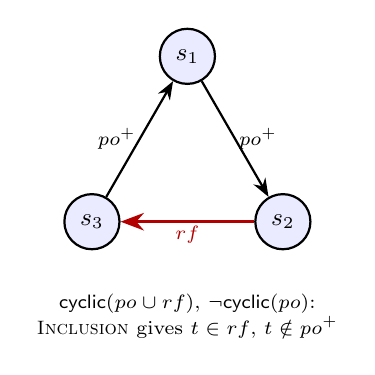
\begin{tikzpicture}
      \foreach \i/\a in {1/90,2/-30,3/210} {
        \node[ev,fill=blue!8] (s\i) at (\a:1.4cm) {$s_{\i}$};
      }
      \draw[arr] (s1) -- node[lab,right]{$po^{+}$} (s2);
      \draw[arr,very thick,red!70!black] (s2) -- node[lab,below]{$rf$} (s3);
      \draw[arr] (s3) -- node[lab,left]{$po^{+}$} (s1);
      \node[font=\scriptsize,align=center] at (0,-1.9)
        {$\cyc{po\cup rf}$, $\neg\cyc{po}$:\\\rn{Inclusion} gives $t\in rf$, $t\notin po^{+}$};
    \end{tikzpicture}
  \end{column}
  \end{columns}
\end{frame}

\begin{frame}{Closure induction (\sm{--rels-tc-subset})}
  \small
  $\TC(R)$ is the least transitive relation that contains $R$:
  \begin{mathpar}
    \inferrule*[right=\rn{TC-Subset}]{(a,b)\in\TC(R) \\ R\subseteq S \\ S;S\subseteq S}{(a,b)\in S}
  \end{mathpar}
  The transitive supersets $S$ recognised in the current context:
  \begin{center}\footnotesize
  \begin{tabular}{@{}L{4.6cm}L{3.9cm}L{5.4cm}@{}}
    \toprule
    superset $S$ & recognised by & example \\
    \midrule
    $\TC(X)$, $R$ syntactically in $\TC(X)$ & the shape of $R$ & $R = po^{+}\cap loc$, $S = po^{+}$ \\
    $S$ transitive, $R\subseteq S$ asserted & $(R\cup S) = S$ in the context &
      $S = A\times B$, a closure, $J;J^T$ with $\fun{J}$ \\
    $R$ itself & $(R;R)\subseteq R$ asserted & $co$ transitive: $\TC(co)=co$ \\
    $R$ itself & $R\subseteq A\times B$, $A\cap B=\emptyset$ & $fr$ from reads to writes: $\TC(fr)=fr$ \\
    $X$, transitive & $R = X\cap Y$ or $R = X\setminus Y$ & \\
    \bottomrule
  \end{tabular}
  \end{center}
  No fresh element: where it applies, one lemma replaces an unbounded descent of \rn{TC-Down}
  splits, each of which introduces two elements. This is what the hand proofs of the
  benchmarks use (``every $ghb$ path is in $po^{+}$'').
\end{frame}

\begin{frame}{Functionality (\sm{--rels-functional-mode})}
  \small
  \begin{mathpar}
    \inferrule*[right=\rn{Fun-UF}]{\fun{R} \\ (x,y)\in S \\ S\sim R}{y = f_R(x)}
    \and
    \inferrule*[right=\rn{Fun-Pairs}]{\fun{R} \\ (x_1,y_1)\in R \\ (x_2,y_2)\in R}{x_1 = x_2 \Rightarrow y_1 = y_2}
    \\
    \inferrule*[right=\rn{Not-Fun}]{\neg\fun{R}}{(k_1,k_2)\in R \wedge (k_1,k_3)\in R \wedge k_2\ne k_3}
  \end{mathpar}
  \begin{itemize}
    \item \sm{uf} (default): a fresh function $f_R$; linear in the members, congruence does the
      rest: $(a,b),(a,c)\in R$ give $b = f_R(a) = c$. \sm{pairs}: quadratic, no function symbol
      (used when the logic has no UF).
    \item With cardinality constraints the solver answers \sm{unknown} (the cardinality solver
      may add members that are not constrained).
    \item Feeds closure induction: $J;J^T$ is transitive if $J$ is functional ($J^T;J$
      relates only equal elements), e.g.\ \emph{same location} $= address;address^T$.
  \end{itemize}
\end{frame}

\begin{frame}{Splitting closures and joins: eager, lazy, or not at all}
  \small
  \textbf{Eager} (cvc5 main): \rn{TC-Down} and \rn{Join-Split} for every membership, each with
  fresh elements. With finite model finding this floods the model with elements.
  \medskip

  \textbf{Lazy} (\sm{--rels-tc-down-lazy}): \rn{TC-Down} only at last call, and only for
  memberships that the known members of $R$ do not explain. Unsat proofs that never unfold a
  closure (closure induction) introduce no element.
  \medskip

  \textbf{Not at all} (\sm{--rels-acyclic-hammer}, for unsat problems): no \rn{TC-Down} and no
  \rn{Join-Split}. At last call a membership that the known members do not explain is a
  conflict:
  \begin{mathpar}
    \inferrule*[right=\rn{Ground-TC}]{(a,b)\in\TC(R) \\ R = \{m_1,\dots,m_n\} \\
      \mathit{distinct}(a,b,\text{elements of the } m_i)}{\bot}
  \end{mathpar}
  and \rn{Ground-Join} for $(x,z)\in A;B$. The distinctness premise matters: without it, the
  conflict for $(a,c)\in A;B$, $A=\{(a,b)\}$, $B=\{(d,c)\}$ refuted the branch $b=d$, in which the
  membership holds (fixed in this PR). With cardinality constraints: \sm{unknown}.
\end{frame}

\begin{frame}{Why inference rules and not rewrite rules?}
  \footnotesize
  \begin{columns}[T]
  \begin{column}{0.4\textwidth}
    \begin{block}{The rewriter}
      maps a term to an \emph{equivalent} term:
      \begin{itemize}
        \item the same in every context (no access to assertions or to the model);
        \item no fresh symbols, no case splits;
        \item terminating, and applied to the input and to every lemma.
      \end{itemize}
      It gets the rules on the term alone: $\cyc{\emptyset}=\bot$,
      $\cyc{\{(x,y)\}} = (x=y)$, constants, closure elimination.
    \end{block}
    Rewriting $\cyc{R}$ to its definition needs a quantifier, or
    $\TC(R)\cap\mathit{iden}(\mathit{univ})\ne\emptyset$, which is wrong in cvc5 (the universe
    is not all elements) and hides the structure the rules use.
  \end{column}
  \begin{column}{0.58\textwidth}
    \scriptsize
    \begin{tabular}{@{}L{3.0cm}L{5.0cm}@{}}
      \toprule
      the rules need & e.g. \\
      \midrule
      a \textbf{witness} (an existential: fresh symbols) & \rn{Cycle-Def}, \rn{Inst-Cycle},
        \rn{Unroll}, \rn{Inclusion}, \rn{Not-Fun} \\
      \textbf{case splits} for the SAT solver & \rn{Unroll} picks an operand,
        \rn{Split-Len} continues or closes \\
      \textbf{other asserted facts} & \rn{TC-Subset} ($R\subseteq S$, $S$ transitive),
        anchors ($\cyc{R}$ and $\neg\cyc{S}$), \rn{Fun-UF} (a membership) \\
      \textbf{equivalence classes} & $S \sim R$, $u\sim R$: premises that hold now, not always \\
      \textbf{the candidate model} & \rn{Branch} ($l = N$), \rn{Ground-TC}, \rn{Ground-Join} \\
      \textbf{unbounded} unfolding & a witness of any length, one element per round \\
      \bottomrule
    \end{tabular}
  \end{column}
  \end{columns}
\end{frame}

\begin{frame}{Soundness}
  \small
  \begin{itemize}
    \item \textbf{Valid lemmas}, consequences of the definitions and the premises: the closure
      rules, \rn{Acyclic-Down}, \rn{Register}, \rn{TC-Subset}, \rn{Fun-Pairs}, and the grounding
      conflicts (thanks to the distinctness premise).
    \item \textbf{Lemmas about skolems}, satisfiability-preserving: any model of the input
      extends to one in which the witness is a shortest cycle of the operands' closures,
      $f_R$ maps every element to its image, etc. This covers \rn{Cycle-Def}, \rn{Inst-Cycle},
      \rn{Unroll}, \rn{Split-Len}, \rn{Alternate}, \rn{Chord}, \rn{Distinct}, \rn{Backward},
      \rn{Inclusion}, \rn{Fun-UF}, \rn{Not-Fun}. \rn{Branch} follows from them (thanks to
      $l = N$).
    \item \textbf{Incompleteness is reported}, so cvc5 answers \sm{unknown} instead of a wrong
      \sm{sat}, when
      \begin{itemize}
        \item the length of a witness has no practical value in the model;
        \item cardinality constraints meet grounding conflicts or \sm{rel.is-functional};
        \item a \sm{rel.rclosure} term is not eliminated by rewriting.
      \end{itemize}
    \item \textbf{Proofs.} The lemmas are trusted theory lemmas; their CPC proofs check with
      ethos (\sm{rel.cyclic}, \sm{rel.is-functional} are in the CPC signature).
  \end{itemize}
\end{frame}

%=====================================================================
\section{Strategy}

\begin{frame}{Where the rules run: cvc5's DPLL($T$) loop}
  \centering
  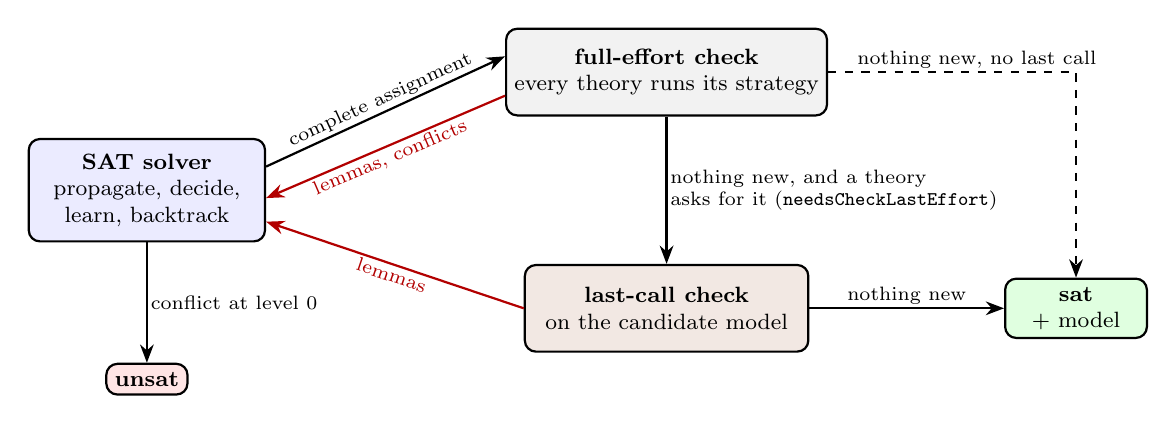
\begin{tikzpicture}
    \node[box,fill=blue!8,minimum width=3.0cm,minimum height=1.3cm] (sat) at (0,0)
      {\textbf{SAT solver}\\propagate, decide,\\learn, backtrack};
    \node[box,fill=gray!10,minimum width=3.6cm,minimum height=1.1cm] (full) at (6.6,1.5)
      {\textbf{full-effort check}\\every theory runs its strategy};
    \node[box,fill=lcc!12,minimum width=3.6cm,minimum height=1.1cm] (last) at (6.6,-1.5)
      {\textbf{last-call check}\\on the candidate model};
    \node[box,fill=green!12,minimum width=1.8cm] (model) at (11.8,-1.5) {\textbf{sat}\\+ model};
    \node[box,fill=red!10] (unsat) at (0,-2.4) {\textbf{unsat}};
    \draw[arr] ([yshift=3mm]sat.east) -- node[lab,above,sloped]{complete assignment}
      ([yshift=2mm]full.west);
    \draw[arr,red!70!black] ([yshift=-3mm]full.west) -- node[lab,below,sloped]{lemmas, conflicts}
      ([yshift=-1mm]sat.east);
    \draw[arr] (full.south) -- node[lab,right,align=left]{nothing new, and a theory\\
      asks for it (\sm{needsCheckLastEffort})} (last.north);
    \draw[arr,red!70!black] (last.west) -- node[lab,below,sloped]{lemmas} ([yshift=-4mm]sat.east);
    \draw[arr] (last.east) -- node[lab,above]{nothing new} (model.west);
    \draw[arr,dashed] (full.east) -| node[lab,above,pos=0.3]{nothing new, no last call}
      (model.north);
    \draw[arr] (sat.south) -- node[lab,right]{conflict at level 0} (unsat.north);
  \end{tikzpicture}
  \medskip

  \small
  \begin{itemize}
    \item The sets theory asks for a last call (\sm{needsCheckLastEffort}) if a cycle witness
      exists, or under \sm{--rels-tc-down-lazy} / \sm{--rels-acyclic-hammer} if closures or
      joins occur.
    \item Lemmas are permanent clauses; the witness and the caches are rolled back on
      backtracking (context-dependent).
  \end{itemize}
\end{frame}

\begin{frame}{The sets strategy at full effort}
  \centering
  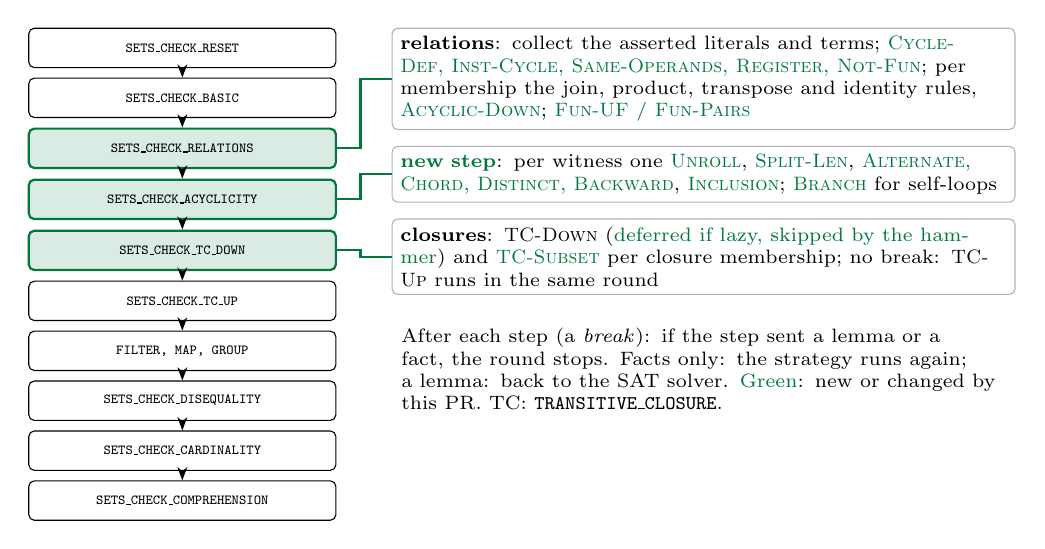
\begin{tikzpicture}[node distance=1.2mm]
    \tikzset{stp/.append style={minimum width=3.9cm,font=\tiny\ttfamily}}
    \node[stp] (reset) {SETS\_CHECK\_RESET};
    \node[stp,below=of reset] (basic) {SETS\_CHECK\_BASIC};
    \node[newstp,below=of basic] (rel) {SETS\_CHECK\_RELATIONS};
    \node[newstp,below=of rel] (acyc) {SETS\_CHECK\_ACYCLICITY};
    \node[newstp,below=of acyc] (down) {SETS\_CHECK\_TC\_DOWN};
    \node[stp,below=of down] (up) {SETS\_CHECK\_TC\_UP};
    \node[stp,below=of up] (fmg) {FILTER, MAP, GROUP};
    \node[stp,below=of fmg] (dis) {SETS\_CHECK\_DISEQUALITY};
    \node[stp,below=of dis] (card) {SETS\_CHECK\_CARDINALITY};
    \node[stp,below=of card] (comp) {SETS\_CHECK\_COMPREHENSION};
    \foreach \a/\b in {reset/basic,basic/rel,rel/acyc,acyc/down,down/up,up/fmg,fmg/dis,dis/card,card/comp} {
      \draw[->,>=Stealth] (\a) -- (\b);
    }
    \node[rules,anchor=north west,text width=7.7cm] (rrel) at ($(reset.north east)+(7mm,0)$)
      {\textbf{relations}: collect the asserted literals and terms; \new{\rn{Cycle-Def},
       \rn{Inst-Cycle}, \rn{Same-Operands}, \rn{Register}, \rn{Not-Fun}}; per membership the join,
       product, transpose and identity rules, \new{\rn{Acyclic-Down}}; \new{\rn{Fun-UF} /
       \rn{Fun-Pairs}}};
    \node[rules,text width=7.7cm,below=2mm of rrel.south west,anchor=north west] (racyc)
      {\textbf{\new{new step}}: per witness one \new{\rn{Unroll}}, \new{\rn{Split-Len}},
       \new{\rn{Alternate}, \rn{Chord}, \rn{Distinct}, \rn{Backward}}, \new{\rn{Inclusion}};
       \new{\rn{Branch}} for self-loops};
    \node[rules,text width=7.7cm,below=2mm of racyc.south west,anchor=north west] (rdown)
      {\textbf{closures}: \rn{TC-Down} (\new{deferred if lazy, skipped by the hammer}) and
       \new{\rn{TC-Subset}} per closure membership; no break: \rn{TC-Up} runs in the same round};
    \draw[newc,thick] (rel.east) -- ++(3mm,0) |- (rrel.west);
    \draw[newc,thick] (acyc.east) -- ++(3mm,0) |- (racyc.west);
    \draw[newc,thick] (down.east) -- ++(3mm,0) |- (rdown.west);
    \node[font=\scriptsize,align=left,anchor=north west,text width=7.7cm] at ($(rdown.south west)+(0,-3mm)$)
      {After each step (a \emph{break}): if the step sent a lemma or a fact, the round stops.
       Facts only: the strategy runs again; a lemma: back to the SAT solver.
       \new{Green}: new or changed by this PR. TC: \sm{TRANSITIVE\_CLOSURE}.};
  \end{tikzpicture}
\end{frame}

\begin{frame}{Last call: the candidate model decides}
  \centering
  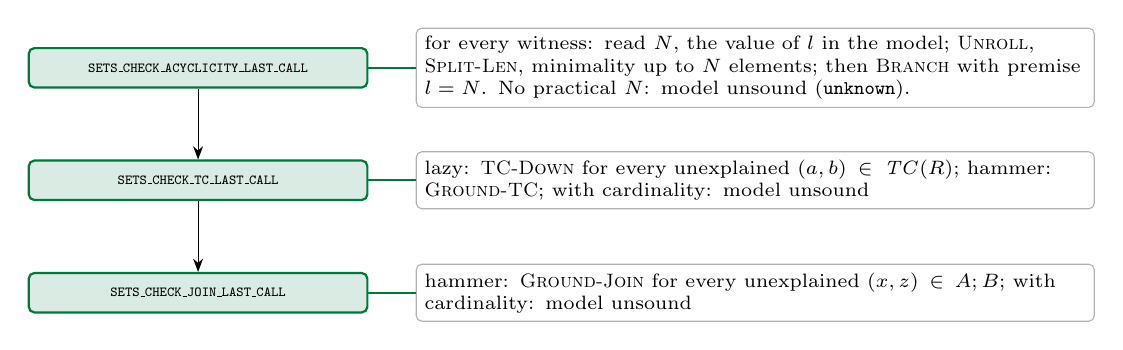
\begin{tikzpicture}[node distance=9mm]
    \tikzset{stp/.append style={font=\tiny\ttfamily}}
    \node[newstp,minimum width=4.3cm] (a) {SETS\_CHECK\_ACYCLICITY\_LAST\_CALL};
    \node[newstp,minimum width=4.3cm,below=of a] (t) {SETS\_CHECK\_TC\_LAST\_CALL};
    \node[newstp,minimum width=4.3cm,below=of t] (j) {SETS\_CHECK\_JOIN\_LAST\_CALL};
    \draw[->,>=Stealth] (a) -- (t);
    \draw[->,>=Stealth] (t) -- (j);
    \node[rules,right=6mm of a,text width=8.4cm] (ra)
      {for every witness: read $N$, the value of $l$ in the model; \rn{Unroll}, \rn{Split-Len},
       minimality up to $N$ elements; then \rn{Branch} with premise $l = N$. No practical $N$:
       model unsound (\sm{unknown}).};
    \node[rules,right=6mm of t,text width=8.4cm] (rt)
      {lazy: \rn{TC-Down} for every unexplained $(a,b)\in\TC(R)$; hammer: \rn{Ground-TC};
       with cardinality: model unsound};
    \node[rules,right=6mm of j,text width=8.4cm] (rj)
      {hammer: \rn{Ground-Join} for every unexplained $(x,z)\in A;B$; with cardinality: model
       unsound};
    \draw[newc,thick] (a) -- (ra);
    \draw[newc,thick] (t) -- (rt);
    \draw[newc,thick] (j) -- (rj);
  \end{tikzpicture}
  \bigskip

  \small
  \begin{itemize}
    \item A step that sends a lemma ends the check; the SAT solver continues with it.
    \item Model-dependent rules belong here: at full effort the length of the witness is still
      symbolic, and the members of a relation are not final.
  \end{itemize}
\end{frame}

\begin{frame}{A cycle witness across the search}
  \centering
  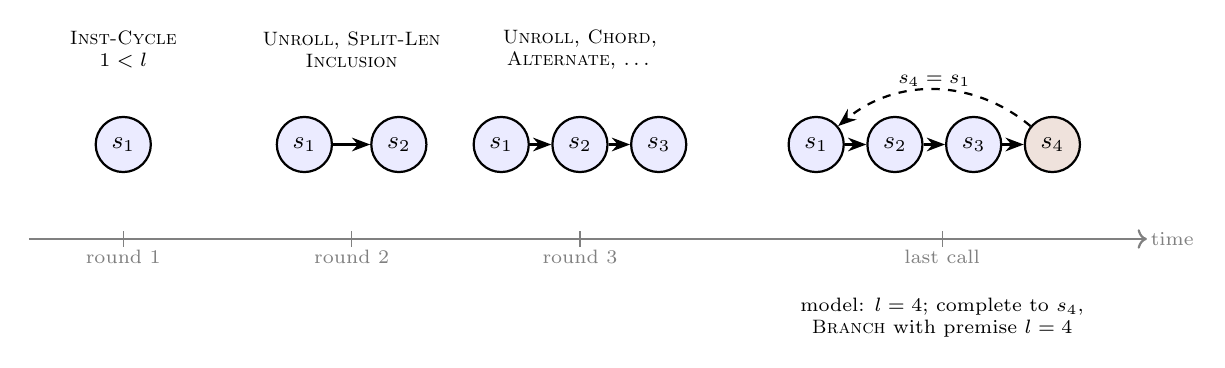
\begin{tikzpicture}[x=1cm,y=1cm]
    \draw[->,thick,gray] (0,0) -- (14.2,0) node[right,lab]{time};
    \foreach \x/\t in {1.2/round 1,4.1/round 2,7.0/round 3,11.6/last call} {
      \draw[gray] (\x,0.1) -- (\x,-0.1) node[below,lab]{\t};
    }
    % round 1
    \node[ev,fill=blue!8] (a1) at (1.2,1.2) {$s_1$};
    \node[lab,align=center] at (1.2,2.4) {\rn{Inst-Cycle}\\$1<l$};
    % round 2
    \node[ev,fill=blue!8] (b1) at (3.5,1.2) {$s_1$};
    \node[ev,fill=blue!8] (b2) at (4.7,1.2) {$s_2$};
    \draw[arr] (b1) -- (b2);
    \node[lab,align=center] at (4.1,2.4) {\rn{Unroll}, \rn{Split-Len}\\\rn{Inclusion}};
    % round 3
    \node[ev,fill=blue!8] (c1) at (6.0,1.2) {$s_1$};
    \node[ev,fill=blue!8] (c2) at (7.0,1.2) {$s_2$};
    \node[ev,fill=blue!8] (c3) at (8.0,1.2) {$s_3$};
    \draw[arr] (c1) -- (c2);
    \draw[arr] (c2) -- (c3);
    \node[lab,align=center] at (7.0,2.4) {\rn{Unroll}, \rn{Chord},\\\rn{Alternate}, \dots};
    % last call
    \node[ev,fill=blue!8] (d1) at (10.0,1.2) {$s_1$};
    \node[ev,fill=blue!8] (d2) at (11.0,1.2) {$s_2$};
    \node[ev,fill=blue!8] (d3) at (12.0,1.2) {$s_3$};
    \node[ev,fill=lcc!15] (d4) at (13.0,1.2) {$s_4$};
    \draw[arr] (d1) -- (d2);
    \draw[arr] (d2) -- (d3);
    \draw[arr] (d3) -- (d4);
    \draw[arr,dashed] (d4) to[bend right=40] node[lab,above]{$s_4 = s_1$} (d1);
    \node[lab,align=center] at (11.6,-1.0) {model: $l = 4$; complete to $s_4$,\\\rn{Branch} with premise $l=4$};
  \end{tikzpicture}
  \bigskip

  \small
  \begin{itemize}
    \item Each round's lemmas go back to the SAT solver; a conflict may backtrack past the
      creation of $s_3$, which then disappears from the witness (and is recreated, as the same
      skolem, if needed again).
    \item A witness that is too long for the problem is refuted by minimality and the anchors;
      a short one survives and its edges become the model's cycle.
  \end{itemize}
\end{frame}

\begin{frame}{Options and defaults}
  \footnotesize
  \begin{tabular}{@{}llL{5.2cm}@{}}
    \toprule
    option & default & effect \\
    \midrule
    \sm{--rels-functional-mode=uf|pairs} & \sm{uf} & how \sm{rel.is-functional} is used \\
    \sm{--rels-acyclic-anchor=branch|inclusion|both|none} & \sm{branch} & anchor rules \\
    \sm{--rels-acyclic-backward-chords} & off & \rn{Backward} (minimality) \\
    \sm{--rels-tc-subset} & off & closure induction \\
    \sm{--rels-tc-down-lazy} & off & \rn{TC-Down} only at last call \\
    \sm{--rels-acyclic-hammer} & off & no \rn{TC-Down} / \rn{Join-Split}; grounding conflicts \\
    \midrule
    \sm{--sets-exp} $\Rightarrow$ MiniSat & on & SAT solver unless set by the user or the
      problem is sygus-style \\
    \bottomrule
  \end{tabular}
  \bigskip

  \small
  All six new options are expert options, off or at their previous behaviour by default. The
  closure rules that need them (closure induction, lazy split, hammer) win on the benchmarks
  only in combination (next section); turning them on by default needs a broader evaluation
  (e.g.\ on cvc5/sets-and-relations-benchmarks).
\end{frame}

%=====================================================================
\section{Results}

\begin{frame}{Setup}
  \scriptsize
  \begin{tabular}{@{}lL{11.8cm}@{}}
    \toprule
    name & options (all on the files without \sm{:finite-model-find}) \\
    \midrule
    default & \sm{--finite-model-find} (as published) \\
    FMF & default + \sm{--e-matching --inst-when=full-delay --rels-acyclic-anchor=inclusion --rels-acyclic-backward-chords} \\
    noFMF & \sm{--rels-acyclic-anchor=inclusion --inst-when=full-delay --rels-acyclic-backward-chords} \\
    stop-only & default + \sm{--decision=stoponly} \\
    FMF+R & FMF + R + \sm{--rels-tc-down-lazy} \\
    noFMF+R & noFMF + R + \sm{--rels-tc-down-lazy} \\
    noFMF+H & noFMF + R + \sm{--rels-acyclic-hammer} \\
    \bottomrule
  \end{tabular}
  \smallskip

  R $=$ \sm{--prenex-quant=none --rels-tc-subset}.
  \smallskip

  \footnotesize
  \begin{itemize}
    \item 13 benchmarks with \sm{rel.cyclic} and \sm{rel.is-functional}
      (relational-solver-benchmarks \pfBench), release build of the branch (\pfCvc), \pfTimeout{} s.
    \item \textbf{Virtual portfolio}: every pair (benchmark, configuration) on its own, \pfJobs{}
      at a time; per benchmark the fastest configuration counts.
    \item \textbf{Real portfolio}: all 7 configurations started together; the first sat/unsat wins.
  \end{itemize}
  \sm{scripts/portfolio.py} runs both modes; \sm{scripts/slides/make\_figures.py} makes the
  following tables and plots.
\end{frame}

\begin{frame}{Every configuration on every benchmark (virtual portfolio)}
  \centering\tiny\setlength{\tabcolsep}{2.6pt}
  \begin{tabular}{@{}lllllllllcl@{}}
\toprule
benchmark & exp. & default & FMF & noFMF & stop-only & FMF+R & noFMF+R & noFMF+H & by & fastest \\
\midrule
sc-1-th & unsat & \tmo & \good{unsat 0.79} & \tmo & \tmo & \good{unsat 0.38} & \best{unsat 0.09} & \tmo & 3 & 0.09 s \\
sc-1-th-just-rf & unsat & \good{unsat 0.20} & \good{unsat 0.15} & \best{unsat 0.05} & \good{unsat 5.24} & \good{unsat 0.09} & \good{unsat 0.05} & \good{unsat 0.05} & 7 & 0.05 s \\
sc-1-th-no-ltts & sat & \best{sat 0.05} & \good{sat 0.09} & \textcolor{orange!80!black}{unknown} & \good{sat 0.14} & \good{sat 0.05} & \textcolor{orange!80!black}{unknown} & \tmo & 4 & 0.05 s \\
sc-2-th & unsat & \tmo & \tmo & \tmo & \tmo & \good{unsat 20.4} & \good{unsat 94.6} & \best{unsat 3.76} & 3 & 3.76 s \\
sc-2-th-just-rf & unsat & \good{unsat 1.10} & \good{unsat 0.38} & \good{unsat 0.25} & \tmo & \good{unsat 0.26} & \good{unsat 0.21} & \best{unsat 0.20} & 6 & 0.20 s \\
plsc-1-th & unsat & \tmo & \good{unsat 5.52} & \tmo & \tmo & \good{unsat 3.97} & \best{unsat 0.95} & \tmo & 3 & 0.95 s \\
plsc-1-th-just-rf & unsat & \tmo & \tmo & \tmo & \tmo & \good{unsat 0.33} & \best{unsat 0.09} & \tmo & 2 & 0.09 s \\
plsc-1-th-no-ltts & sat & \good{sat 0.09} & \good{sat 0.14} & \textcolor{orange!80!black}{unknown} & \good{sat 0.38} & \best{sat 0.08} & \textcolor{orange!80!black}{unknown} & \tmo & 4 & 0.08 s \\
plsc-2-th & unsat & \tmo & \tmo & \tmo & \tmo & \tmo & \best{unsat 75.8} & \tmo & 1 & 75.8 s \\
plsc-2-th-just-rf & unsat & \tmo & \tmo & \tmo & \tmo & \good{unsat 1.08} & \best{unsat 0.38} & \tmo & 2 & 0.38 s \\
tso-1-th & unsat & \tmo & \tmo & \tmo & \tmo & \good{unsat 288.7} & \best{unsat 6.87} & \tmo & 2 & 6.87 s \\
tso-1-th-just-rf & unsat & \tmo & \good{unsat 5.64} & \tmo & \tmo & \good{unsat 0.27} & \best{unsat 0.09} & \tmo & 3 & 0.09 s \\
tso-1-th-no-ltts & sat & \good{sat 4.44} & \tmo & \textcolor{orange!80!black}{unknown} & \tmo & \best{sat 1.22} & \tmo & \tmo & 2 & 1.22 s \\
\midrule
solved & & 5 & 7 & 2 & 3 & 12 & 10 & 3 & \multicolumn{2}{l}{\textbf{13 of 13}} \\
\bottomrule
\end{tabular}

  \medskip

  {\raggedright\scriptsize \pfTimeout{} s per run. Bold: the fastest configuration, which the
  virtual best takes. ``by'': how many configurations solve the file. \pfWrong{} wrong answers.
  The best single configuration (\pfBestSingleName) solves \pfBestSingle{}; the portfolio solves
  \textbf{\pfVirtual{} of \pfTotal}. plsc-2-th is solved by noFMF+R only.\par}
\end{frame}

\begin{frame}{The portfolio as a cactus plot}
  \centering
  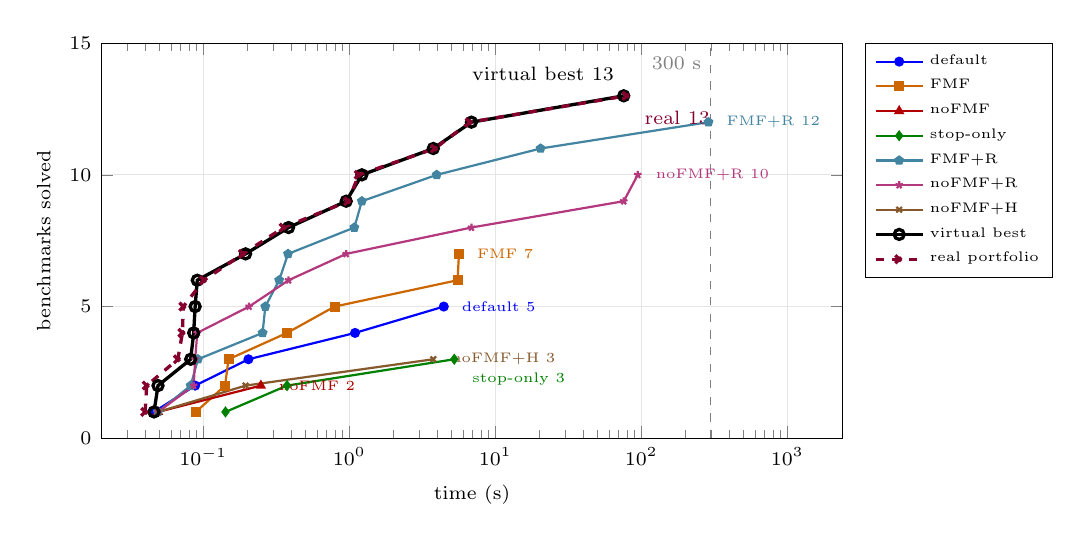
\begin{tikzpicture}
    \begin{axis}[width=11cm, height=6.6cm, xmode=log, xmin=0.02, xmax=2400,
  xlabel={time (s)}, ylabel={benchmarks solved}, ymin=0, ymax=15,
  tick label style={font=\scriptsize}, label style={font=\scriptsize},
  legend style={font=\tiny,at={(1.03,1)},anchor=north west}, legend cell align=left,
  grid=major, grid style={gray!20}]
\addplot[thick,blue,mark=*,mark size=1.4pt] coordinates {(0.046,1) (0.088,2) (0.204,3) (1.096,4) (4.441,5)};
\addlegendentry{default}
\addplot[thick,orange!80!black,mark=square*,mark size=1.4pt] coordinates {(0.089,1) (0.141,2) (0.149,3) (0.375,4) (0.794,5) (5.519,6) (5.64,7)};
\addlegendentry{FMF}
\addplot[thick,red!70!black,mark=triangle*,mark size=1.4pt] coordinates {(0.049,1) (0.248,2)};
\addlegendentry{noFMF}
\addplot[thick,green!50!black,mark=diamond*,mark size=1.4pt] coordinates {(0.142,1) (0.375,2) (5.239,3)};
\addlegendentry{stop-only}
\addplot[thick,cyan!60!black,mark=pentagon*,mark size=1.4pt] coordinates {(0.049,1) (0.082,2) (0.092,3) (0.255,4) (0.266,5) (0.331,6) (0.381,7) (1.083,8) (1.22,9) (3.974,10) (20.433,11) (288.729,12)};
\addlegendentry{FMF+R}
\addplot[thick,magenta!70!black,mark=star,mark size=1.4pt] coordinates {(0.049,1) (0.086,2) (0.088,3) (0.091,4) (0.206,5) (0.384,6) (0.953,7) (6.867,8) (75.845,9) (94.636,10)};
\addlegendentry{noFMF+R}
\addplot[thick,brown!70!black,mark=x,mark size=1.4pt] coordinates {(0.049,1) (0.195,2) (3.763,3)};
\addlegendentry{noFMF+H}
\addplot[very thick,black,mark=o,mark size=1.8pt] coordinates {(0.046,1) (0.049,2) (0.082,3) (0.086,4) (0.088,5) (0.091,6) (0.195,7) (0.384,8) (0.953,9) (1.22,10) (3.763,11) (6.867,12) (75.845,13)};
\addlegendentry{virtual best}
\addplot[very thick,purple!70!black,dashed,mark=x,mark size=2pt] coordinates {(0.04,1) (0.041,2) (0.067,3) (0.072,4) (0.073,5) (0.101,6) (0.187,7) (0.355,8) (0.983,9) (1.161,10) (3.857,11) (6.686,12) (79.349,13)};
\addlegendentry{real portfolio}
\draw[dashed,gray] (axis cs:300,0) -- (axis cs:300,15) node[pos=0.95,left,font=\scriptsize]{300 s};
\node[font=\tiny,red!70!black,anchor=west,xshift=3pt,yshift=0pt] at (axis cs:0.248,2) {noFMF 2};
\node[font=\tiny,brown!70!black,anchor=west,xshift=3pt,yshift=0pt] at (axis cs:3.763,3) {noFMF+H 3};
\node[font=\tiny,green!50!black,anchor=west,xshift=3pt,yshift=-7pt] at (axis cs:5.239,3) {stop-only 3};
\node[font=\tiny,blue,anchor=west,xshift=3pt,yshift=0pt] at (axis cs:4.441,5) {default 5};
\node[font=\tiny,orange!80!black,anchor=west,xshift=3pt,yshift=0pt] at (axis cs:5.64,7) {FMF 7};
\node[font=\tiny,magenta!70!black,anchor=west,xshift=3pt,yshift=0pt] at (axis cs:94.636,10) {noFMF+R 10};
\node[font=\tiny,cyan!60!black,anchor=west,xshift=3pt,yshift=0pt] at (axis cs:288.729,12) {FMF+R 12};
\node[font=\scriptsize,anchor=south east,yshift=2pt] at (axis cs:75.845,13) {virtual best 13};
\node[font=\scriptsize,purple!70!black,anchor=north west,xshift=3pt,yshift=-2pt] at (axis cs:79.349,13) {real 13};
\end{axis}

  \end{tikzpicture}\\
  \footnotesize Each curve: one configuration's solve times, sorted; cumulative count; final count at
  its right end. Virtual best: per file the fastest configuration. Real: all \pfNumConfigs{}
  started together.
\end{frame}

\begin{frame}{Virtual best versus real portfolio}
  \begin{columns}[T]
  \begin{column}{0.56\textwidth}
    \tiny\setlength{\tabcolsep}{3pt}
    \begin{tabular}{@{}llrrr@{}}
\toprule
benchmark & winner & VBS & real & CPU \\
\midrule
sc-1-th & noFMF+R & 0.09 s & 0.06 s & 0.4 s \\
sc-1-th-just-rf & noFMF & 0.05 s & 0.06 s & 0.3 s \\
sc-1-th-no-ltts & default & 0.05 s & 0.04 s & 0.2 s \\
sc-2-th & noFMF+H & 3.85 s & 3.86 s & 27.0 s \\
sc-2-th-just-rf & noFMF+H / noFMF+R & 0.21 s & 0.19 s & 1.2 s \\
plsc-1-th & noFMF+R & 0.96 s & 0.95 s & 6.7 s \\
plsc-1-th-just-rf & noFMF+R & 0.09 s & 0.09 s & 0.6 s \\
plsc-1-th-no-ltts & default & 0.09 s & 0.09 s & 0.6 s \\
plsc-2-th & noFMF+R & 76.9 s & 79.5 s & 556.4 s \\
plsc-2-th-just-rf & noFMF+R & 0.38 s & 0.35 s & 2.5 s \\
tso-1-th & noFMF+R & 7.14 s & 6.86 s & 48.0 s \\
tso-1-th-just-rf & noFMF+R & 0.08 s & 0.09 s & 0.5 s \\
tso-1-th-no-ltts & FMF+R & 1.27 s & 1.19 s & 7.1 s \\
\bottomrule
\end{tabular}

    \medskip

    \scriptsize Virtual: \pfVirtual{} of \pfTotal{}. Real: \pfReal{} of \pfTotal{}, with the same winner on
    \pfSame{}; real/virtual between \pfRatioMin{} and \pfRatioMax{} (median \pfRatioMed). Ratios
    below 1: the virtual runs also share the CPU (\pfJobs{} at a time).
  \end{column}
  \begin{column}{0.42\textwidth}
    \centering
    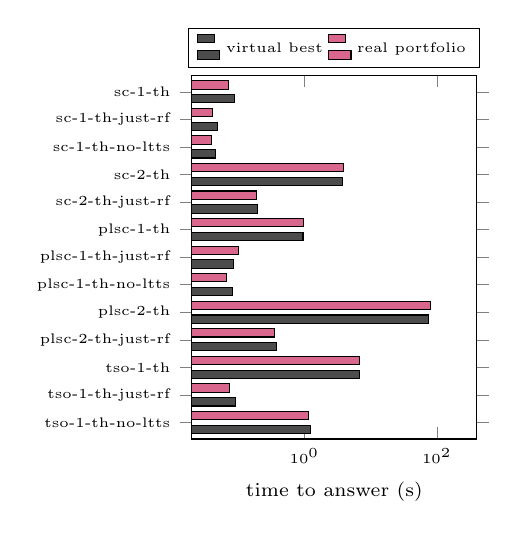
\begin{tikzpicture}
      \begin{axis}[xbar, width=5.2cm, height=6.2cm, xmode=log, log origin=infty,
  symbolic y coords={sc-1-th,sc-1-th-just-rf,sc-1-th-no-ltts,sc-2-th,sc-2-th-just-rf,plsc-1-th,plsc-1-th-just-rf,plsc-1-th-no-ltts,plsc-2-th,plsc-2-th-just-rf,tso-1-th,tso-1-th-just-rf,tso-1-th-no-ltts}, ytick=data, y dir=reverse,
  tick label style={font=\tiny}, xlabel={time to answer (s)}, xlabel style={font=\scriptsize},
  xmin=0.02, xmax=400, bar width=3pt, enlarge y limits=0.05,
  legend style={font=\tiny,at={(0.5,1.02)},anchor=south,legend columns=2}]
\addplot[fill=black!70] coordinates {(0.088,sc-1-th) (0.049,sc-1-th-just-rf) (0.046,sc-1-th-no-ltts) (3.763,sc-2-th) (0.195,sc-2-th-just-rf) (0.953,plsc-1-th) (0.086,plsc-1-th-just-rf) (0.082,plsc-1-th-no-ltts) (75.845,plsc-2-th) (0.384,plsc-2-th-just-rf) (6.867,tso-1-th) (0.091,tso-1-th-just-rf) (1.22,tso-1-th-no-ltts)};
\addplot[fill=purple!60] coordinates {(0.072,sc-1-th) (0.041,sc-1-th-just-rf) (0.04,sc-1-th-no-ltts) (3.857,sc-2-th) (0.187,sc-2-th-just-rf) (0.983,plsc-1-th) (0.101,plsc-1-th-just-rf) (0.067,plsc-1-th-no-ltts) (79.349,plsc-2-th) (0.355,plsc-2-th-just-rf) (6.686,tso-1-th) (0.073,tso-1-th-just-rf) (1.161,tso-1-th-no-ltts)};
\legend{virtual best, real portfolio}
\end{axis}

    \end{tikzpicture}\\
    \scriptsize Every real answer within \pfMaxReal{} s. plsc-2-th needs 53 s on a fast
    core, 286 s on an efficiency core.
  \end{column}
  \end{columns}
\end{frame}

\begin{frame}{Testing}
  \footnotesize
  \begin{itemize}
    \item \textbf{Regressions}: 53 new or changed files; all 443 sets, relations and bags
      regressions and all 2800 \sm{regress0} tests pass with assertions on.
    \item \textbf{Proofs}: the CPC proofs of all 84 applicable unsat relations regressions check
      with ethos; \sm{garbage\_collect.cvc} times out, as on main. The check found that
      \sm{rel.rclosure}, \sm{rel.rtclosure} were missing from the CPC signature (added).
    \item \textbf{Fuzzing} against brute force: 5\,500 random problems
      (\sm{rel.cyclic} of unions, nested either way, \sm{(not (rel.cyclic S))}, pairs forced in,
      out, or free) under five option sets: no wrong answer, no error.
    \item \textbf{Bugs found on the way, fixed in this PR}:
      \begin{itemize}
        \item the join grounding conflict refuted satisfiable branches under the hammer (missing
          distinctness);
        \item \sm{rel.rclosure} of a union crashed debug builds, and of a variable answered
          \sm{sat} wrongly (now \sm{unknown});
        \item the MiniSat default answered \sm{unsat} wrongly with \sm{:produce-interpolants} (a
          latent issue, also on main with \sm{--sat-solver=minisat}); the default now skips
          sygus-style problems.
      \end{itemize}
    \item \textbf{CI}: formatting (clang-format 22, whole files) and the CPC/Logos check pass.
  \end{itemize}
\end{frame}

%=====================================================================
\section{Summary}

\begin{frame}{Contributions}
  \begin{itemize}
    \item Two predicates for relational specifications, \sm{rel.cyclic} and
      \sm{rel.is-functional}, with API, parser, printer, type rules, rewrites, CPC declarations and
      documentation.
    \item A calculus for them in the relations solver:
      \begin{itemize}
        \item a cycle witness that is a shortest cycle of the operands' closures, unrolled
          one element per round and completed from the model;
        \item acyclicity, and anchors that connect cyclic and acyclic constraints;
        \item closure induction, which proves closure memberships without fresh elements;
        \item functionality by a skolem function;
        \item lazy and grounded closure reasoning.
      \end{itemize}
    \item A strategy that places each rule: context rules at full effort, model-dependent rules
      at last call.
    \item On the 13 litmus-template benchmarks: \textbf{13 of 13} solved by the portfolio
      (virtual and real), no wrong answer.
  \end{itemize}
\end{frame}

\begin{frame}{Where to find it}
  \small
  \begin{itemize}
    \item PR to cvc5 main: \sm{mudathirmahgoub/cvc5\#17} (branch \sm{cycle-ext-cyclic}); the same
      branch is \sm{rachelcleaveland/cvc5\#9}, stacked on the earlier \sm{cycle-ext} PRs.
    \item Benchmarks: \sm{rachelcleaveland/relational-solver-benchmarks}, directories
      \sm{benchmarks-ltts} and \sm{benchmarks-ltts-nofmf}.
    \item Temporary, to be deleted before merging: \sm{scripts/} (portfolio runner, ablation,
      comparison, converters) and \sm{scripts/slides/} (this deck, its figure generator and the
      run data).
    \item Rebuild the deck: \sm{cd scripts/slides; python3 make\_figures.py data/final-300s
      figures; pdflatex relations-pr.tex}.
  \end{itemize}
\end{frame}

\end{document}
